\section{Data-Science Experiment Results}\label{app:datascience-results}

This appendix gives the optimizer steps and additional failure diagnostics
for the local-search comparison in
Section~\ref{subsec:black-box-datascience-finite-budget-optimization}.
Sampling definitions and statistical results are presented with their
interpretation in Section~\ref{sec:black-box-datascience}.

\subsection{Finite-budget local optimizer comparison}

The run configuration labels the \(64\) starting bodies as held out.
The saved hashes identify the seven configurations used, but do not establish
that these bodies were absent from earlier development or tuning. A later
development configuration reuses \(16\) starts. Their earlier selection history
is therefore unresolved; this does not show that the reported outcomes were
used to select the configurations.

Every run used the same allocation rule: a nominal \(1000\)\,ms
start-new-work cutoff for charged full-evaluator plus optimizer time and a cap
of \(128\) full historical-evaluator calls.  In-progress work could complete
atomically past the cutoff, and methods could terminate early, so realized
compute differs across runs.  The \(448\) traces contain \(28824\) full calls.
Using the historical numerical objective described in
Section~\ref{subsec:black-box-datascience-finite-budget-optimization},
four-anchor branch history has the largest comparison-block median best value,
\(0.9848\), followed by transition prediction at \(0.9816\) and the finite-gap
affine model at \(0.9772\).  No run reaches
a recorded numerical ratio of one.

\paragraph{The implemented optimizer steps.}
Except for the literal gradient, the methods remove the fifteen infinitesimal
symmetry directions from the forty dual-normal coordinates. The local models
and coordinate poll recompute this transverse space at their anchors;
CMA-ES keeps its initial space. The literal gradient uses the ambient
coordinates.  Every
outer proposal is checked by a fresh geometry reconstruction and the
configured full orbit-word search.  The implementations below are frozen
comparison points; their parameters are not claimed to optimize the
corresponding algorithm families.

\begingroup
\small
\begin{longtable}{@{}p{0.24\linewidth}p{0.67\linewidth}@{}}
\caption{One outer iteration of each optimizer in the recorded
comparison.}
\label{tab:black-box-datascience-f10-optimizer-steps}\\
\toprule
method & implemented step\\
\midrule
\endfirsthead
\toprule
method & implemented step\\
\midrule
\endhead
literal and safeguarded branch gradients
& Differentiate one currently minimizing branch.  The literal method takes
  \(a^+=a+0.01D_as_\sigma(a)\) even after a decrease.  The safeguarded method
  projects and normalizes this gradient, accepts only a fully evaluated
  improvement, and expands or halves its distance after acceptance or
  rejection.\\
finite-gap affine model
& Keep the current branch gaps in a \(10\%\) action window, linearize their
  values, and maximize the minimum affine value on a local ball.  Fully
  evaluate the proposal and use the same expand-or-halve distance rule.\\
four-anchor branch history
& Union candidate words from the four most recent full searches, using a
  \(30\%\) action window and normalized beta allowance \(0.3\).  At a nearby
  point, re-solve the named KKT branches, discard transition-infeasible and
  beta-inadmissible solutions, linearize the remaining values, and maximize
  their affine minimum.  Take at most two internal moves before the next full
  evaluation.\\
history with transition prediction
& Use the preceding method, but for a normalized internal move of length at
  least \(0.08\), also predict newly feasible transitions in the move
  direction and evaluate the words thereby generated.\\
CMA-ES
& Fully evaluate a population of eight Gaussian perturbations, then update
  the mean, covariance, and normalized scale from their ranking.\\
coordinate direct search
& Poll both signs of the \(25\) transverse basis axes.  Move to the best
  improvement and double the radius, or halve the radius if no poll point
  improves.\\
\bottomrule
\end{longtable}
\endgroup

The companion endpoint packet does not test local maximality.  Signed polls
along the transverse basis find an improving direction at seven of \(16\)
one-second branch-history endpoints and two of the corresponding five-second
endpoints.  Separate validated continuation paths show that even an endpoint
with no improving basis direction can retain appreciable ascent between the
tested axes.  These observations diagnose insufficient finite budgets; they
do not estimate the distance to a local maximum.

\paragraph{Detailed HKO calibration.}
On \(16\) known perturbations along four development directions from HKO, the
multi-branch continuation accepted no move at HKO and improved every
perturbation.  One step recovered \(93.4\%\)--\(100\%\) of the known evaluator
gap and removed \(77.9\%\)--\(100\%\) of the distance to HKO.  In contrast,
the gradient of one current minimizing branch recovered
\(-22.1\%\)--\(41.4\%\) of the gap.

\begin{figure}[htbp]
\centering
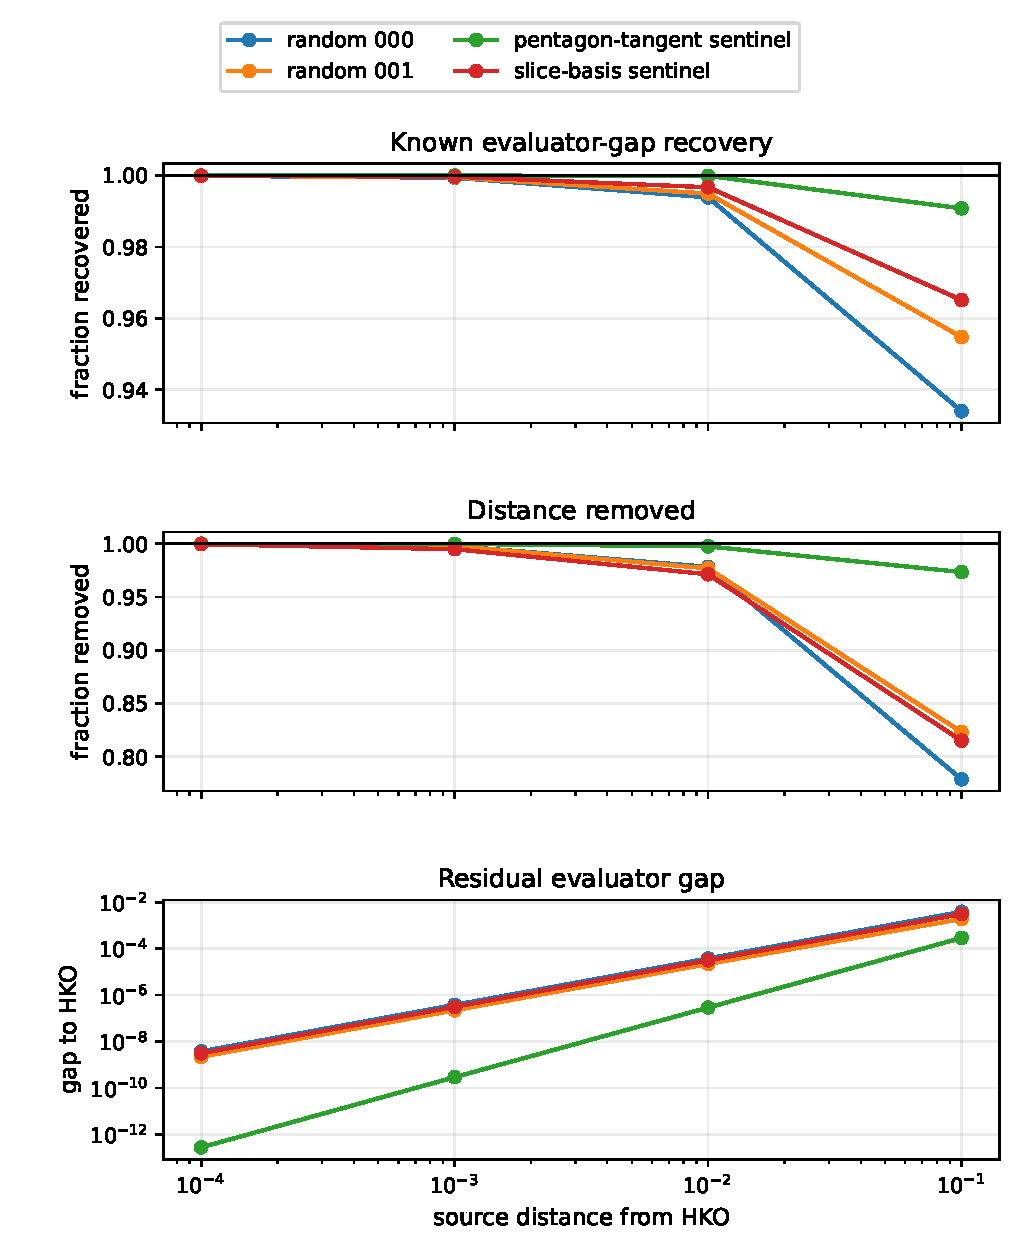
\includegraphics[width=\linewidth]
  {figures/datascience/hko-recovery-by-source-distance.pdf}
\caption{One-step calibration on known perturbations of HKO.  From top to
bottom, the panels show recovered evaluator gap, removed distance, and
residual evaluator gap.}
\label{fig:black-box-datascience-hko-optimizer-calibration}
\end{figure}

\paragraph{Selected finite-step failure audit.}
At the eight highest four-anchor tuning endpoints, five admitted one validated
improvement, by \(1.57\cdot10^{-6}\) to \(4.61\cdot10^{-5}\).  Across the
\(80\) multi-branch proposals, \(52\) decreased the recomputed evaluator value
despite a represented target winner and positive affine prediction; \(40\) of
these losses retained determinate, unchanged geometry.  All \(40\)
current-branch gradient proposals decreased.

The three-proposal audit compared two such failures with one positive control.
At normalized radius \(10^{-5}\), the failures perturbed their named KKT
matrices by \(218\) and \(67\) times the smallest base eigenvalue magnitude
and crossed zero; the control had ratio \(1.53\), did not cross zero, and kept
the correct sign.  At the smallest tested radius, \(10^{-8}\), central
differences approximated the implemented analytic derivatives with relative
errors below \(1\%\) for the named action and \(1.9\%\) for the named branch
ratio.  Binary64 and exact-arithmetic geometry
reconstruction agreed at all \(39\) audited points, and relative volume
discrepancies were below \(10^{-15}\).  For these selected cases the observed
failure is finite-distance nonlinearity of an ill-conditioned KKT branch.

\begin{figure}[htbp]
\centering
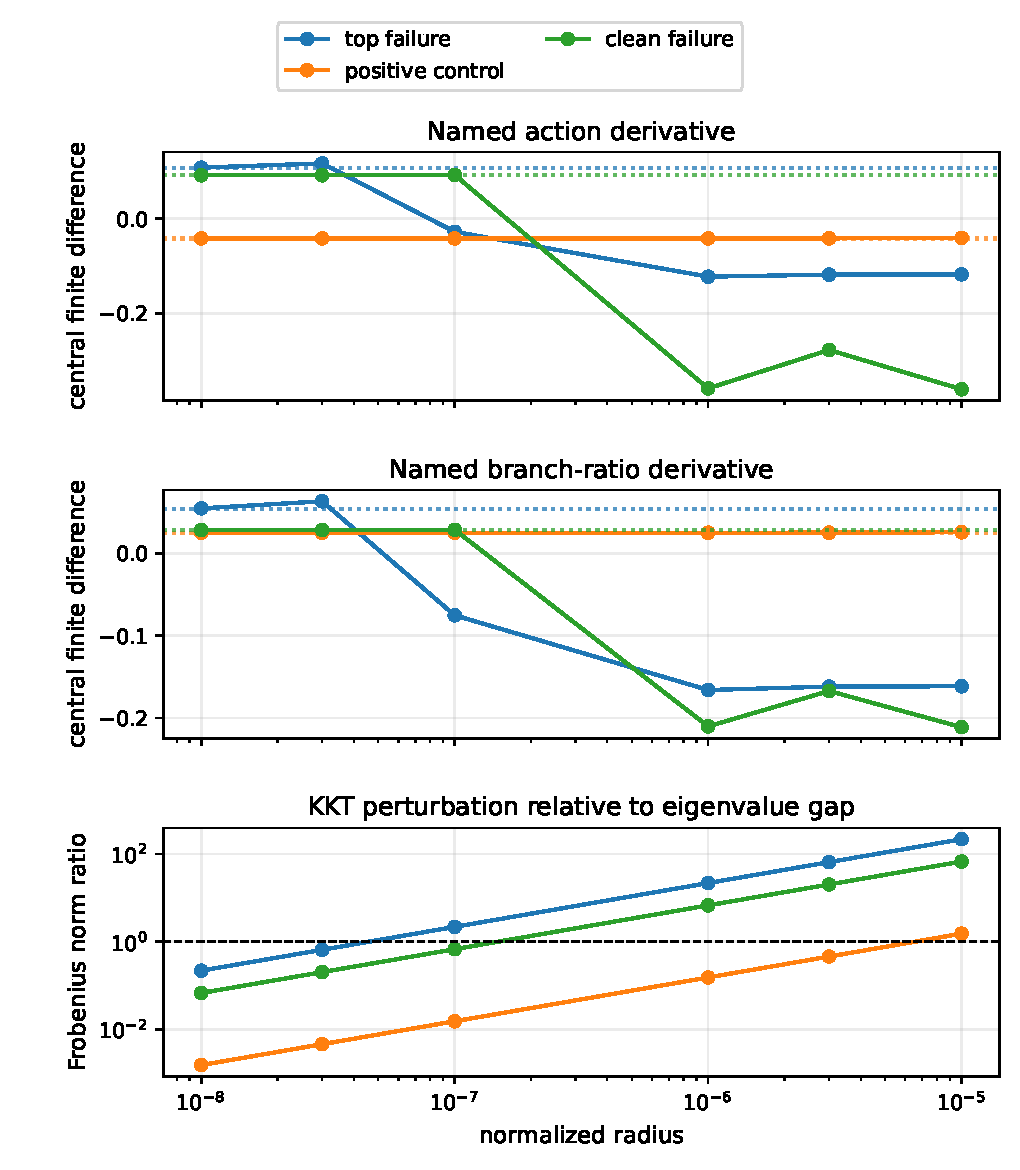
\includegraphics[width=\linewidth]
  {figures/datascience/derivative-and-kkt-scale.pdf}
\caption{Finite differences for two failed affine proposals and one positive
control.  Prediction changes regime when the KKT perturbation becomes large
relative to the smallest source eigenvalue magnitude (bottom).  Dotted lines
in the top two panels are the analytic derivatives.}
\label{fig:black-box-datascience-kkt-trust-scale}
\end{figure}

These diagnostics use selected controls rather than population samples.  They
do not provide a convergence theorem, a population error rate, or a universal
conditioning cutoff.
